%!TEX root = *.tex
%%%%%%%%%%%%%%%%%%
% カウンタのリセット
\setcounter{figure}{0}
% 問題文
{
\begin{wrapfigure}{r}{22zw}
  \vspace{-\intextsep}
  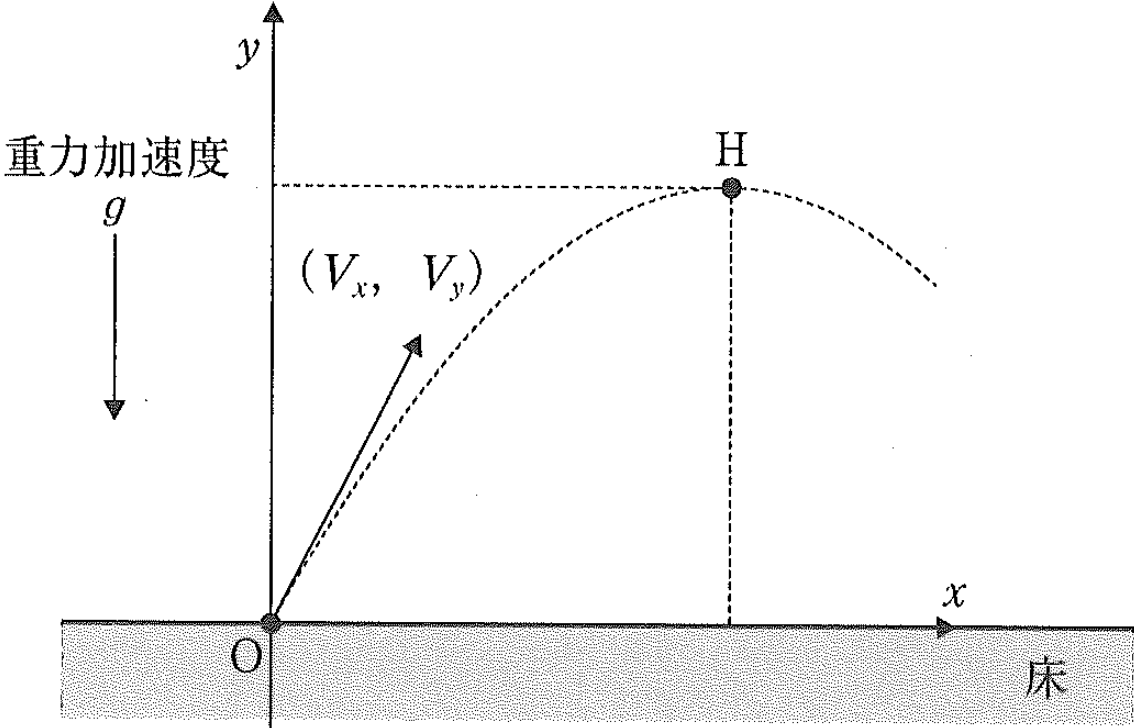
\includegraphics[width=22zw]{../graphs/noko_23_1.png}
  \caption{}
\end{wrapfigure}

なめらかで水平な床について,図1に示すように,原点Oおよび水平右向きに\x 軸,鉛直方向上向きに\y 軸を定める.
いま,質量$m$の小物体を原点Oから\xy 平面内において斜め上方に打ち出す.
この打ち出した瞬間の速度成分を,\x 方向,\y 方向それぞれについて$V_x$,$V_y$であるとする.
この小物体は鉛直下向きに一定の大きさ$mg$の重力を受けながら運動し,何度も床と衝突してはねかえる.
このとき,小物体と床の衝突は非弾性衝突であり,反発係数$e$は$0<e<1$である.
ただし,この小物体に対する空気抵抗は無視できるとする.
この小物体の運動について以下の問いに答えよ.
なお,解答において用いてよい文字は,特に指定がなければ$g,\,m,\,V_x,\,V_y$および$e$である.

\par}

\begin{enumerate}[(1)]
  \setlength{\leftskip}{-1zw}
  \setlength{\itemindent}{1zw}\setlength{\labelsep}{0.5zw}
  \setlength{\labelwidth}{1zw}\setlength{\leftmargin}{1zw}
  \setlength{\itemsep}{0.5\baselineskip}
  \item 小物体が打ち出されてから床と最初に衝突するまでの間における最高到達点Hの\x 座標,\y 座標をそれぞれ答えよ.
  \item 小物体が打ち出されてから床と最初に衝突する点を$\text{P}_1$とする.点$\text{P}_1$においてはねかえった直後の小物体の速度の\x 成分,\y 成分をそれぞれ答えよ.
  \item 点$\text{P}_1$における衝突において,小物体が失った力学的エネルギー$\varDelta E_1$を答えよ.
  \item 小物体が打ち出されてから床と2回目に衝突する点を$\text{P}_2$とする.点$\text{P}_2$における衝突において,小物体が失った力学的エネルギー$\varDelta E_2$を答えよ.
  \item 小物体が打ち出されてから床と$n$回目に衝突する点を$\text{P}_n$とする.点$\text{P}_n$における衝突において,小物体が失った力学的エネルギー$\varDelta E_n$を答えよ.ただし,この答えには,問題文はじめに指定した文字に加えて$n$を用いてよい.
  \item 小物体が打ち出されてから床と最初に衝突するまでの間における最高到達点Hの衝突回数が十分に大きくなると,小物体の衝突直後の速度は最終的に一定となる.この一定となった速度の\x 成分,\y 成分をそれぞれ答えよ.
  \item 小物体が打ち出されてから床と$n$回目に衝突するまでに失った力学的エネルギーの総和について考える.床との衝突回数が十分に大きくなると,この総和は最終的にある値となる.この値を答えよ.
\end{enumerate}





% メモ
\begin{comment}

\end{comment}


%%%%%%%%%%%%%%%%%%
